\documentclass[1p]{elsarticle_modified}
%\bibliographystyle{elsarticle-num}

%\usepackage[colorlinks]{hyperref}
%\usepackage{abbrmath_seonhwa} %\Abb, \Ascr, \Acal ,\Abf, \Afrak
\usepackage{amsfonts}
\usepackage{amssymb}
\usepackage{amsmath}
\usepackage{amsthm}
\usepackage{scalefnt}
\usepackage{amsbsy}
\usepackage{kotex}
\usepackage{caption}
\usepackage{subfig}
\usepackage{color}
\usepackage{graphicx}
\usepackage{xcolor} %% white, black, red, green, blue, cyan, magenta, yellow
\usepackage{float}
\usepackage{setspace}
\usepackage{hyperref}

\usepackage{tikz}
\usetikzlibrary{arrows}

\usepackage{multirow}
\usepackage{array} % fixed length table
\usepackage{hhline}

%%%%%%%%%%%%%%%%%%%%%
\makeatletter
\renewcommand*\env@matrix[1][\arraystretch]{%
	\edef\arraystretch{#1}%
	\hskip -\arraycolsep
	\let\@ifnextchar\new@ifnextchar
	\array{*\c@MaxMatrixCols c}}
\makeatother %https://tex.stackexchange.com/questions/14071/how-can-i-increase-the-line-spacing-in-a-matrix
%%%%%%%%%%%%%%%

\usepackage[normalem]{ulem}

\newcommand{\msout}[1]{\ifmmode\text{\sout{\ensuremath{#1}}}\else\sout{#1}\fi}
%SOURCE: \msout is \stkout macro in https://tex.stackexchange.com/questions/20609/strikeout-in-math-mode

\newcommand{\cancel}[1]{
	\ifmmode
	{\color{red}\msout{#1}}
	\else
	{\color{red}\sout{#1}}
	\fi
}

\newcommand{\add}[1]{
	{\color{blue}\uwave{#1}}
}

\newcommand{\replace}[2]{
	\ifmmode
	{\color{red}\msout{#1}}{\color{blue}\uwave{#2}}
	\else
	{\color{red}\sout{#1}}{\color{blue}\uwave{#2}}
	\fi
}

\newcommand{\Sol}{\mathcal{S}} %segment
\newcommand{\D}{D} %diagram
\newcommand{\A}{\mathcal{A}} %arc


%%%%%%%%%%%%%%%%%%%%%%%%%%%%%5 test

\def\sl{\operatorname{\textup{SL}}(2,\Cbb)}
\def\psl{\operatorname{\textup{PSL}}(2,\Cbb)}
\def\quan{\mkern 1mu \triangleright \mkern 1mu}

\theoremstyle{definition}
\newtheorem{thm}{Theorem}[section]
\newtheorem{prop}[thm]{Proposition}
\newtheorem{lem}[thm]{Lemma}
\newtheorem{ques}[thm]{Question}
\newtheorem{cor}[thm]{Corollary}
\newtheorem{defn}[thm]{Definition}
\newtheorem{exam}[thm]{Example}
\newtheorem{rmk}[thm]{Remark}
\newtheorem{alg}[thm]{Algorithm}

\newcommand{\I}{\sqrt{-1}}
\begin{document}

%\begin{frontmatter}
%
%\title{Boundary parabolic representations of knots up to 8 crossings}
%
%%% Group authors per affiliation:
%\author{Yunhi Cho} 
%\address{Department of Mathematics, University of Seoul, Seoul, Korea}
%\ead{yhcho@uos.ac.kr}
%
%
%\author{Seonhwa Kim} %\fnref{s_kim}}
%\address{Center for Geometry and Physics, Institute for Basic Science, Pohang, 37673, Korea}
%\ead{ryeona17@ibs.re.kr}
%
%\author{Hyuk Kim}
%\address{Department of Mathematical Sciences, Seoul National University, Seoul 08826, Korea}
%\ead{hyukkim@snu.ac.kr}
%
%\author{Seokbeom Yoon}
%\address{Department of Mathematical Sciences, Seoul National University, Seoul, 08826,  Korea}
%\ead{sbyoon15@snu.ac.kr}
%
%\begin{abstract}
%We find all boundary parabolic representation of knots up to 8 crossings.
%
%\end{abstract}
%\begin{keyword}
%    \MSC[2010] 57M25 
%\end{keyword}
%
%\end{frontmatter}

%\linenumbers
%\tableofcontents
%
\newcommand\colored[1]{\textcolor{white}{\rule[-0.35ex]{0.8em}{1.4ex}}\kern-0.8em\color{red} #1}%
%\newcommand\colored[1]{\textcolor{white}{ #1}\kern-2.17ex	\textcolor{white}{ #1}\kern-1.81ex	\textcolor{white}{ #1}\kern-2.15ex\color{red}#1	}

{\Large $\underline{12a_{0751}~(K12a_{0751})}$}

\setlength{\tabcolsep}{10pt}
\renewcommand{\arraystretch}{1.6}
\vspace{1cm}\begin{tabular}{m{100pt}>{\centering\arraybackslash}m{274pt}}
\multirow{5}{120pt}{
	\centering
	\includegraphics[width=112pt]{../../../GIT/diagram.site/Diagrams/png/1552_12a_0751.png}\\
\ \ \ A knot diagram\footnotemark}&
\allowdisplaybreaks
\textbf{Linearized knot diagam} \\
\cline{2-2}
 &
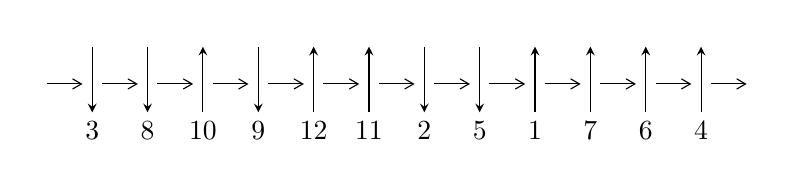
\begin{tikzpicture}[x=20pt, y=17pt]
	% nodes
	\node (C0) at (0, 0) {};
	\node (C1) at (1, 0) {};
	\node (C1U) at (1, +1) {};
	\node (C1D) at (1, -1) {3};

	\node (C2) at (2, 0) {};
	\node (C2U) at (2, +1) {};
	\node (C2D) at (2, -1) {8};

	\node (C3) at (3, 0) {};
	\node (C3U) at (3, +1) {};
	\node (C3D) at (3, -1) {10};

	\node (C4) at (4, 0) {};
	\node (C4U) at (4, +1) {};
	\node (C4D) at (4, -1) {9};

	\node (C5) at (5, 0) {};
	\node (C5U) at (5, +1) {};
	\node (C5D) at (5, -1) {12};

	\node (C6) at (6, 0) {};
	\node (C6U) at (6, +1) {};
	\node (C6D) at (6, -1) {11};

	\node (C7) at (7, 0) {};
	\node (C7U) at (7, +1) {};
	\node (C7D) at (7, -1) {2};

	\node (C8) at (8, 0) {};
	\node (C8U) at (8, +1) {};
	\node (C8D) at (8, -1) {5};

	\node (C9) at (9, 0) {};
	\node (C9U) at (9, +1) {};
	\node (C9D) at (9, -1) {1};

	\node (C10) at (10, 0) {};
	\node (C10U) at (10, +1) {};
	\node (C10D) at (10, -1) {7};

	\node (C11) at (11, 0) {};
	\node (C11U) at (11, +1) {};
	\node (C11D) at (11, -1) {6};

	\node (C12) at (12, 0) {};
	\node (C12U) at (12, +1) {};
	\node (C12D) at (12, -1) {4};
	\node (C13) at (13, 0) {};

	% arrows
	\draw[->,>={angle 60}]
	(C0) edge (C1) (C1) edge (C2) (C2) edge (C3) (C3) edge (C4) (C4) edge (C5) (C5) edge (C6) (C6) edge (C7) (C7) edge (C8) (C8) edge (C9) (C9) edge (C10) (C10) edge (C11) (C11) edge (C12) (C12) edge (C13) ;	\draw[->,>=stealth]
	(C1U) edge (C1D) (C2U) edge (C2D) (C3D) edge (C3U) (C4U) edge (C4D) (C5D) edge (C5U) (C6D) edge (C6U) (C7U) edge (C7D) (C8U) edge (C8D) (C9D) edge (C9U) (C10D) edge (C10U) (C11D) edge (C11U) (C12D) edge (C12U) ;
	\end{tikzpicture} \\
\hhline{~~} \\& 
\textbf{Solving Sequence} \\ \cline{2-2} 
 &
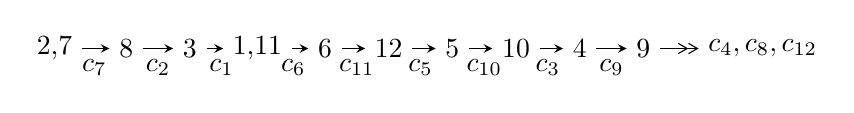
\begin{tikzpicture}[x=23pt, y=7pt]
	% node
	\node (A0) at (-1/8, 0) {2,7};
	\node (A1) at (1, 0) {8};
	\node (A2) at (2, 0) {3};
	\node (A3) at (49/16, 0) {1,11};
	\node (A4) at (33/8, 0) {6};
	\node (A5) at (41/8, 0) {12};
	\node (A6) at (49/8, 0) {5};
	\node (A7) at (57/8, 0) {10};
	\node (A8) at (65/8, 0) {4};
	\node (A9) at (73/8, 0) {9};
	\node (C1) at (1/2, -1) {$c_{7}$};
	\node (C2) at (3/2, -1) {$c_{2}$};
	\node (C3) at (5/2, -1) {$c_{1}$};
	\node (C4) at (29/8, -1) {$c_{6}$};
	\node (C5) at (37/8, -1) {$c_{11}$};
	\node (C6) at (45/8, -1) {$c_{5}$};
	\node (C7) at (53/8, -1) {$c_{10}$};
	\node (C8) at (61/8, -1) {$c_{3}$};
	\node (C9) at (69/8, -1) {$c_{9}$};
	\node (A10) at (11, 0) {$c_{4},c_{8},c_{12}$};

	% edge
	\draw[->,>=stealth]	
	(A0) edge (A1) (A1) edge (A2) (A2) edge (A3) (A3) edge (A4) (A4) edge (A5) (A5) edge (A6) (A6) edge (A7) (A7) edge (A8) (A8) edge (A9) ;
	\draw[->>,>={angle 60}]	
	(A9) edge (A10);
\end{tikzpicture} \\ 

\end{tabular} \\

\footnotetext{
The image of knot diagram is generated by the software ``\textbf{Draw programme}" developed by Andrew Bartholomew(\url{http://www.layer8.co.uk/maths/draw/index.htm\#Running-draw}), where we modified some parts for our purpose(\url{https://github.com/CATsTAILs/LinksPainter}).
}\phantom \\ \newline 
\centering \textbf{Ideals for irreducible components\footnotemark of $X_{\text{par}}$} 
 
\begin{align*}
I^u_{1}&=\langle 
5.59626\times10^{121} u^{99}+7.57270\times10^{121} u^{98}+\cdots+1.04618\times10^{122} b+1.03099\times10^{124},\\
\phantom{I^u_{1}}&\phantom{= \langle  }3.41104\times10^{123} u^{99}+1.78701\times10^{123} u^{98}+\cdots+1.15079\times10^{123} a+4.33722\times10^{125},\\
\phantom{I^u_{1}}&\phantom{= \langle  }u^{100}+u^{99}+\cdots+192 u+88\rangle \\
I^u_{2}&=\langle 
- u^{17}- u^{16}+\cdots+b-4,\;u^{19}- u^{18}+\cdots+a-5,\;u^{20}-5 u^{18}+\cdots- u+1\rangle \\
\\
\end{align*}
\raggedright * 2 irreducible components of $\dim_{\mathbb{C}}=0$, with total 120 representations.\\
\footnotetext{All coefficients of polynomials are rational numbers. But the coefficients are sometimes approximated in decimal forms when there is not enough margin.}
\newpage
\renewcommand{\arraystretch}{1}
\centering \section*{I. $I^u_{1}= \langle 5.60\times10^{121} u^{99}+7.57\times10^{121} u^{98}+\cdots+1.05\times10^{122} b+1.03\times10^{124},\;3.41\times10^{123} u^{99}+1.79\times10^{123} u^{98}+\cdots+1.15\times10^{123} a+4.34\times10^{125},\;u^{100}+u^{99}+\cdots+192 u+88 \rangle$}
\flushleft \textbf{(i) Arc colorings}\\
\begin{tabular}{m{7pt} m{180pt} m{7pt} m{180pt} }
\flushright $a_{2}=$&$\begin{pmatrix}0\\u\end{pmatrix}$ \\
\flushright $a_{7}=$&$\begin{pmatrix}1\\0\end{pmatrix}$ \\
\flushright $a_{8}=$&$\begin{pmatrix}1\\u^2\end{pmatrix}$ \\
\flushright $a_{3}=$&$\begin{pmatrix}- u\\- u^3+u\end{pmatrix}$ \\
\flushright $a_{1}=$&$\begin{pmatrix}u^3\\u^5- u^3+u\end{pmatrix}$ \\
\flushright $a_{11}=$&$\begin{pmatrix}-2.96408 u^{99}-1.55285 u^{98}+\cdots-374.031 u-376.889\\-0.534925 u^{99}-0.723846 u^{98}+\cdots-84.1661 u-98.5485\end{pmatrix}$ \\
\flushright $a_{6}=$&$\begin{pmatrix}0.617617 u^{99}-1.17346 u^{98}+\cdots+37.6546 u-38.2669\\2.51995 u^{99}-0.410169 u^{98}+\cdots+285.419 u+168.064\end{pmatrix}$ \\
\flushright $a_{12}=$&$\begin{pmatrix}2.09671 u^{99}+1.08332 u^{98}+\cdots+250.069 u+258.434\\1.72681 u^{99}+0.999934 u^{98}+\cdots+237.814 u+210.154\end{pmatrix}$ \\
\flushright $a_{5}=$&$\begin{pmatrix}-2.27990 u^{99}+1.58306 u^{98}+\cdots-240.947 u-25.0792\\-3.87185 u^{99}-0.0865608 u^{98}+\cdots-443.404 u-309.362\end{pmatrix}$ \\
\flushright $a_{10}=$&$\begin{pmatrix}-2.42915 u^{99}-0.829001 u^{98}+\cdots-289.865 u-278.341\\-0.534925 u^{99}-0.723846 u^{98}+\cdots-84.1661 u-98.5485\end{pmatrix}$ \\
\flushright $a_{4}=$&$\begin{pmatrix}-0.845112 u^{99}+0.558376 u^{98}+\cdots-83.0591 u-2.45370\\-1.36008 u^{99}+0.253366 u^{98}+\cdots-116.779 u-81.9261\end{pmatrix}$ \\
\flushright $a_{9}=$&$\begin{pmatrix}-2.85480 u^{99}-1.37610 u^{98}+\cdots-351.640 u-359.046\\-0.790636 u^{99}-0.977449 u^{98}+\cdots-118.031 u-144.290\end{pmatrix}$\\&\end{tabular}
\flushleft \textbf{(ii) Obstruction class $= -1$}\\~\\
\flushleft \textbf{(iii) Cusp Shapes $= -3.86987 u^{99}-0.145177 u^{98}+\cdots-447.994 u-326.668$}\\~\\
\newpage\renewcommand{\arraystretch}{1}
\flushleft \textbf{(iv) u-Polynomials at the component}\newline \\
\begin{tabular}{m{50pt}|m{274pt}}
Crossings & \hspace{64pt}u-Polynomials at each crossing \\
\hline $$\begin{aligned}c_{1}\end{aligned}$$&$\begin{aligned}
&u^{100}+45 u^{99}+\cdots+119584 u+7744
\end{aligned}$\\
\hline $$\begin{aligned}c_{2},c_{7}\end{aligned}$$&$\begin{aligned}
&u^{100}+u^{99}+\cdots+192 u+88
\end{aligned}$\\
\hline $$\begin{aligned}c_{3}\end{aligned}$$&$\begin{aligned}
&u^{100}+3 u^{98}+\cdots+1720 u+379
\end{aligned}$\\
\hline $$\begin{aligned}c_{4},c_{8}\end{aligned}$$&$\begin{aligned}
&u^{100}+2 u^{99}+\cdots+2370 u+1621
\end{aligned}$\\
\hline $$\begin{aligned}c_{5},c_{6},c_{10}\\c_{11}\end{aligned}$$&$\begin{aligned}
&u^{100}- u^{99}+\cdots+6 u+1
\end{aligned}$\\
\hline $$\begin{aligned}c_{9}\end{aligned}$$&$\begin{aligned}
&u^{100}-3 u^{99}+\cdots+566 u+1753
\end{aligned}$\\
\hline $$\begin{aligned}c_{12}\end{aligned}$$&$\begin{aligned}
&u^{100}+9 u^{99}+\cdots+45 u+1
\end{aligned}$\\
\hline
\end{tabular}\\~\\
\newpage\renewcommand{\arraystretch}{1}
\flushleft \textbf{(v) Riley Polynomials at the component}\newline \\
\begin{tabular}{m{50pt}|m{274pt}}
Crossings & \hspace{64pt}Riley Polynomials at each crossing \\
\hline $$\begin{aligned}c_{1}\end{aligned}$$&$\begin{aligned}
&y^{100}+31 y^{99}+\cdots+454960640 y+59969536
\end{aligned}$\\
\hline $$\begin{aligned}c_{2},c_{7}\end{aligned}$$&$\begin{aligned}
&y^{100}-45 y^{99}+\cdots-119584 y+7744
\end{aligned}$\\
\hline $$\begin{aligned}c_{3}\end{aligned}$$&$\begin{aligned}
&y^{100}+6 y^{99}+\cdots+2142182 y+143641
\end{aligned}$\\
\hline $$\begin{aligned}c_{4},c_{8}\end{aligned}$$&$\begin{aligned}
&y^{100}+62 y^{99}+\cdots+49983400 y+2627641
\end{aligned}$\\
\hline $$\begin{aligned}c_{5},c_{6},c_{10}\\c_{11}\end{aligned}$$&$\begin{aligned}
&y^{100}+121 y^{99}+\cdots+32 y+1
\end{aligned}$\\
\hline $$\begin{aligned}c_{9}\end{aligned}$$&$\begin{aligned}
&y^{100}-31 y^{99}+\cdots-158167488 y+3073009
\end{aligned}$\\
\hline $$\begin{aligned}c_{12}\end{aligned}$$&$\begin{aligned}
&y^{100}+y^{99}+\cdots-499 y+1
\end{aligned}$\\
\hline
\end{tabular}\\~\\
\newpage\flushleft \textbf{(vi) Complex Volumes and Cusp Shapes}
$$\begin{array}{c|c|c}  
\text{Solutions to }I^u_{1}& \I (\text{vol} + \sqrt{-1}CS) & \text{Cusp shape}\\
 \hline 
\begin{aligned}
u &= \phantom{-}0.457128 + 0.895092 I \\
a &= \phantom{-}0.277346 - 0.131143 I \\
b &= -0.591223 - 0.738873 I\end{aligned}
 & \phantom{-}3.20370 + 8.08248 I & \phantom{-0.000000 } 0 \\ \hline\begin{aligned}
u &= \phantom{-}0.457128 - 0.895092 I \\
a &= \phantom{-}0.277346 + 0.131143 I \\
b &= -0.591223 + 0.738873 I\end{aligned}
 & \phantom{-}3.20370 - 8.08248 I & \phantom{-0.000000 } 0 \\ \hline\begin{aligned}
u &= -0.949475 + 0.353004 I \\
a &= -0.0965409 - 0.0295078 I \\
b &= -0.501613 + 0.333772 I\end{aligned}
 & -1.61218 + 1.26315 I & \phantom{-0.000000 } 0 \\ \hline\begin{aligned}
u &= -0.949475 - 0.353004 I \\
a &= -0.0965409 + 0.0295078 I \\
b &= -0.501613 - 0.333772 I\end{aligned}
 & -1.61218 - 1.26315 I & \phantom{-0.000000 } 0 \\ \hline\begin{aligned}
u &= \phantom{-}0.487153 + 0.858326 I \\
a &= -0.411419 + 0.471713 I \\
b &= \phantom{-}0.08719 + 1.60914 I\end{aligned}
 & -8.68625 + 4.27677 I & \phantom{-0.000000 } 0 \\ \hline\begin{aligned}
u &= \phantom{-}0.487153 - 0.858326 I \\
a &= -0.411419 - 0.471713 I \\
b &= \phantom{-}0.08719 - 1.60914 I\end{aligned}
 & -8.68625 - 4.27677 I & \phantom{-0.000000 } 0 \\ \hline\begin{aligned}
u &= -0.811221 + 0.558161 I \\
a &= -0.610382 - 0.676529 I \\
b &= \phantom{-}0.456846 - 0.636360 I\end{aligned}
 & \phantom{-}2.56446 - 0.54418 I & \phantom{-0.000000 } 0 \\ \hline\begin{aligned}
u &= -0.811221 - 0.558161 I \\
a &= -0.610382 + 0.676529 I \\
b &= \phantom{-}0.456846 + 0.636360 I\end{aligned}
 & \phantom{-}2.56446 + 0.54418 I & \phantom{-0.000000 } 0 \\ \hline\begin{aligned}
u &= -0.909159 + 0.370130 I \\
a &= \phantom{-}1.00785 - 2.56119 I \\
b &= \phantom{-}0.04380 - 1.79990 I\end{aligned}
 & -12.07290 + 1.51771 I & \phantom{-0.000000 } 0 \\ \hline\begin{aligned}
u &= -0.909159 - 0.370130 I \\
a &= \phantom{-}1.00785 + 2.56119 I \\
b &= \phantom{-}0.04380 + 1.79990 I\end{aligned}
 & -12.07290 - 1.51771 I & \phantom{-0.000000 } 0\\
 \hline 
 \end{array}$$\newpage$$\begin{array}{c|c|c}  
\text{Solutions to }I^u_{1}& \I (\text{vol} + \sqrt{-1}CS) & \text{Cusp shape}\\
 \hline 
\begin{aligned}
u &= -0.943267 + 0.393422 I \\
a &= -1.16845 + 1.06220 I \\
b &= \phantom{-}0.549467 + 0.827812 I\end{aligned}
 & -1.80876 + 1.49561 I & \phantom{-0.000000 } 0 \\ \hline\begin{aligned}
u &= -0.943267 - 0.393422 I \\
a &= -1.16845 - 1.06220 I \\
b &= \phantom{-}0.549467 - 0.827812 I\end{aligned}
 & -1.80876 - 1.49561 I & \phantom{-0.000000 } 0 \\ \hline\begin{aligned}
u &= \phantom{-}0.049849 + 1.035490 I \\
a &= -0.119703 - 1.284840 I \\
b &= -0.07255 - 1.55357 I\end{aligned}
 & -3.35710 + 0.84569 I & \phantom{-0.000000 } 0 \\ \hline\begin{aligned}
u &= \phantom{-}0.049849 - 1.035490 I \\
a &= -0.119703 + 1.284840 I \\
b &= -0.07255 + 1.55357 I\end{aligned}
 & -3.35710 - 0.84569 I & \phantom{-0.000000 } 0 \\ \hline\begin{aligned}
u &= -0.345894 + 0.892402 I \\
a &= \phantom{-}0.043148 + 0.616596 I \\
b &= -0.378598 + 0.534759 I\end{aligned}
 & \phantom{-}3.66695 + 0.64439 I & \phantom{-0.000000 } 0 \\ \hline\begin{aligned}
u &= -0.345894 - 0.892402 I \\
a &= \phantom{-}0.043148 - 0.616596 I \\
b &= -0.378598 - 0.534759 I\end{aligned}
 & \phantom{-}3.66695 - 0.64439 I & \phantom{-0.000000 } 0 \\ \hline\begin{aligned}
u &= -0.875061 + 0.578879 I \\
a &= \phantom{-}1.12333 - 1.91481 I \\
b &= -0.313739 - 0.731171 I\end{aligned}
 & \phantom{-}2.36569 + 5.08929 I & \phantom{-0.000000 } 0 \\ \hline\begin{aligned}
u &= -0.875061 - 0.578879 I \\
a &= \phantom{-}1.12333 + 1.91481 I \\
b &= -0.313739 + 0.731171 I\end{aligned}
 & \phantom{-}2.36569 - 5.08929 I & \phantom{-0.000000 } 0 \\ \hline\begin{aligned}
u &= -0.971552 + 0.444847 I \\
a &= -2.90650 + 2.58483 I \\
b &= \phantom{-}0.01149 + 1.56483 I\end{aligned}
 & -6.12144 - 1.12485 I & \phantom{-0.000000 } 0 \\ \hline\begin{aligned}
u &= -0.971552 - 0.444847 I \\
a &= -2.90650 - 2.58483 I \\
b &= \phantom{-}0.01149 - 1.56483 I\end{aligned}
 & -6.12144 + 1.12485 I & \phantom{-0.000000 } 0\\
 \hline 
 \end{array}$$\newpage$$\begin{array}{c|c|c}  
\text{Solutions to }I^u_{1}& \I (\text{vol} + \sqrt{-1}CS) & \text{Cusp shape}\\
 \hline 
\begin{aligned}
u &= \phantom{-}1.068870 + 0.136323 I \\
a &= -0.01112 - 1.51128 I \\
b &= -0.228583 - 0.936404 I\end{aligned}
 & -5.43132 + 1.06691 I & \phantom{-0.000000 } 0 \\ \hline\begin{aligned}
u &= \phantom{-}1.068870 - 0.136323 I \\
a &= -0.01112 + 1.51128 I \\
b &= -0.228583 + 0.936404 I\end{aligned}
 & -5.43132 - 1.06691 I & \phantom{-0.000000 } 0 \\ \hline\begin{aligned}
u &= -0.532098 + 0.746302 I \\
a &= \phantom{-}0.624469 - 0.643270 I \\
b &= -0.754980 - 0.223997 I\end{aligned}
 & \phantom{-}4.77059 - 3.60253 I & \phantom{-0.000000 } 0 \\ \hline\begin{aligned}
u &= -0.532098 - 0.746302 I \\
a &= \phantom{-}0.624469 + 0.643270 I \\
b &= -0.754980 + 0.223997 I\end{aligned}
 & \phantom{-}4.77059 + 3.60253 I & \phantom{-0.000000 } 0 \\ \hline\begin{aligned}
u &= \phantom{-}0.901590 + 0.137482 I \\
a &= -0.225698 - 0.574004 I \\
b &= \phantom{-}0.656804 + 0.210978 I\end{aligned}
 & \phantom{-}0.01670 + 2.78694 I & \phantom{-0.000000 } 0 \\ \hline\begin{aligned}
u &= \phantom{-}0.901590 - 0.137482 I \\
a &= -0.225698 + 0.574004 I \\
b &= \phantom{-}0.656804 - 0.210978 I\end{aligned}
 & \phantom{-}0.01670 - 2.78694 I & \phantom{-0.000000 } 0 \\ \hline\begin{aligned}
u &= -0.407065 + 1.010870 I \\
a &= \phantom{-}0.255522 + 0.839954 I \\
b &= -0.17440 + 1.62012 I\end{aligned}
 & -4.76816 - 10.95720 I & \phantom{-0.000000 } 0 \\ \hline\begin{aligned}
u &= -0.407065 - 1.010870 I \\
a &= \phantom{-}0.255522 - 0.839954 I \\
b &= -0.17440 - 1.62012 I\end{aligned}
 & -4.76816 + 10.95720 I & \phantom{-0.000000 } 0 \\ \hline\begin{aligned}
u &= \phantom{-}0.973821 + 0.494263 I \\
a &= \phantom{-}2.07761 + 3.20985 I \\
b &= -0.09275 + 1.62754 I\end{aligned}
 & -5.79792 - 6.63756 I & \phantom{-0.000000 } 0 \\ \hline\begin{aligned}
u &= \phantom{-}0.973821 - 0.494263 I \\
a &= \phantom{-}2.07761 - 3.20985 I \\
b &= -0.09275 - 1.62754 I\end{aligned}
 & -5.79792 + 6.63756 I & \phantom{-0.000000 } 0\\
 \hline 
 \end{array}$$\newpage$$\begin{array}{c|c|c}  
\text{Solutions to }I^u_{1}& \I (\text{vol} + \sqrt{-1}CS) & \text{Cusp shape}\\
 \hline 
\begin{aligned}
u &= \phantom{-}0.982131 + 0.534639 I \\
a &= \phantom{-}0.573213 + 0.834066 I \\
b &= \phantom{-}0.550859 + 1.189730 I\end{aligned}
 & -0.83659 - 3.90380 I & \phantom{-0.000000 } 0 \\ \hline\begin{aligned}
u &= \phantom{-}0.982131 - 0.534639 I \\
a &= \phantom{-}0.573213 - 0.834066 I \\
b &= \phantom{-}0.550859 - 1.189730 I\end{aligned}
 & -0.83659 + 3.90380 I & \phantom{-0.000000 } 0 \\ \hline\begin{aligned}
u &= \phantom{-}0.480220 + 0.730326 I \\
a &= -0.391373 - 0.230176 I \\
b &= -0.05183 - 1.60666 I\end{aligned}
 & -8.61603 - 0.90830 I & \phantom{-0.000000 } 0 \\ \hline\begin{aligned}
u &= \phantom{-}0.480220 - 0.730326 I \\
a &= -0.391373 + 0.230176 I \\
b &= -0.05183 + 1.60666 I\end{aligned}
 & -8.61603 + 0.90830 I & \phantom{-0.000000 } 0 \\ \hline\begin{aligned}
u &= \phantom{-}0.790912 + 0.351475 I \\
a &= -2.42436 - 1.13611 I \\
b &= \phantom{-}0.040636 - 0.416164 I\end{aligned}
 & \phantom{-}0.88125 + 1.31215 I & \phantom{-0.000000 } 0 \\ \hline\begin{aligned}
u &= \phantom{-}0.790912 - 0.351475 I \\
a &= -2.42436 + 1.13611 I \\
b &= \phantom{-}0.040636 + 0.416164 I\end{aligned}
 & \phantom{-}0.88125 - 1.31215 I & \phantom{-0.000000 } 0 \\ \hline\begin{aligned}
u &= -1.055800 + 0.416304 I \\
a &= -0.477868 + 0.407449 I \\
b &= -0.501700 + 0.764707 I\end{aligned}
 & -2.26962 + 1.47318 I & \phantom{-0.000000 } 0 \\ \hline\begin{aligned}
u &= -1.055800 - 0.416304 I \\
a &= -0.477868 - 0.407449 I \\
b &= -0.501700 - 0.764707 I\end{aligned}
 & -2.26962 - 1.47318 I & \phantom{-0.000000 } 0 \\ \hline\begin{aligned}
u &= \phantom{-}1.023140 + 0.506583 I \\
a &= \phantom{-}0.579107 + 0.555358 I \\
b &= -0.471189 - 0.035664 I\end{aligned}
 & -0.45591 - 4.68155 I & \phantom{-0.000000 } 0 \\ \hline\begin{aligned}
u &= \phantom{-}1.023140 - 0.506583 I \\
a &= \phantom{-}0.579107 - 0.555358 I \\
b &= -0.471189 + 0.035664 I\end{aligned}
 & -0.45591 + 4.68155 I & \phantom{-0.000000 } 0\\
 \hline 
 \end{array}$$\newpage$$\begin{array}{c|c|c}  
\text{Solutions to }I^u_{1}& \I (\text{vol} + \sqrt{-1}CS) & \text{Cusp shape}\\
 \hline 
\begin{aligned}
u &= \phantom{-}0.662351 + 0.538131 I \\
a &= \phantom{-}1.43717 + 1.53013 I \\
b &= -0.400932 + 1.267270 I\end{aligned}
 & \phantom{-}0.179494 - 0.448818 I & \phantom{-0.000000 } 0 \\ \hline\begin{aligned}
u &= \phantom{-}0.662351 - 0.538131 I \\
a &= \phantom{-}1.43717 - 1.53013 I \\
b &= -0.400932 - 1.267270 I\end{aligned}
 & \phantom{-}0.179494 + 0.448818 I & \phantom{-0.000000 } 0 \\ \hline\begin{aligned}
u &= -0.480432 + 0.704035 I \\
a &= -0.720306 + 0.070361 I \\
b &= \phantom{-}0.311817 - 0.699242 I\end{aligned}
 & -0.75596 - 2.78991 I & \phantom{-0.000000 -}0. + 5.33071 I \\ \hline\begin{aligned}
u &= -0.480432 - 0.704035 I \\
a &= -0.720306 - 0.070361 I \\
b &= \phantom{-}0.311817 + 0.699242 I\end{aligned}
 & -0.75596 + 2.78991 I & \phantom{-0.000000 } 0. - 5.33071 I \\ \hline\begin{aligned}
u &= \phantom{-}0.919034 + 0.695465 I \\
a &= -0.388402 + 0.015091 I \\
b &= \phantom{-}0.450194 - 0.156366 I\end{aligned}
 & \phantom{-}3.85181 - 2.66231 I & \phantom{-0.000000 } 0 \\ \hline\begin{aligned}
u &= \phantom{-}0.919034 - 0.695465 I \\
a &= -0.388402 - 0.015091 I \\
b &= \phantom{-}0.450194 + 0.156366 I\end{aligned}
 & \phantom{-}3.85181 + 2.66231 I & \phantom{-0.000000 } 0 \\ \hline\begin{aligned}
u &= \phantom{-}1.061530 + 0.451220 I \\
a &= \phantom{-}0.64755 + 1.28489 I \\
b &= -0.686878 + 0.598970 I\end{aligned}
 & -2.00804 - 5.39813 I & \phantom{-0.000000 } 0 \\ \hline\begin{aligned}
u &= \phantom{-}1.061530 - 0.451220 I \\
a &= \phantom{-}0.64755 - 1.28489 I \\
b &= -0.686878 - 0.598970 I\end{aligned}
 & -2.00804 + 5.39813 I & \phantom{-0.000000 } 0 \\ \hline\begin{aligned}
u &= \phantom{-}0.855748 + 0.776003 I \\
a &= -0.059404 + 0.560020 I \\
b &= -0.147280 - 0.150368 I\end{aligned}
 & \phantom{-}4.15579 - 3.00585 I & \phantom{-0.000000 } 0 \\ \hline\begin{aligned}
u &= \phantom{-}0.855748 - 0.776003 I \\
a &= -0.059404 - 0.560020 I \\
b &= -0.147280 + 0.150368 I\end{aligned}
 & \phantom{-}4.15579 + 3.00585 I & \phantom{-0.000000 } 0\\
 \hline 
 \end{array}$$\newpage$$\begin{array}{c|c|c}  
\text{Solutions to }I^u_{1}& \I (\text{vol} + \sqrt{-1}CS) & \text{Cusp shape}\\
 \hline 
\begin{aligned}
u &= \phantom{-}0.699689 + 0.447370 I \\
a &= -0.85775 + 1.47416 I \\
b &= \phantom{-}0.12893 + 1.57137 I\end{aligned}
 & -4.86721 + 2.69174 I & \phantom{-}2.00000 + 3.09443 I \\ \hline\begin{aligned}
u &= \phantom{-}0.699689 - 0.447370 I \\
a &= -0.85775 - 1.47416 I \\
b &= \phantom{-}0.12893 - 1.57137 I\end{aligned}
 & -4.86721 - 2.69174 I & \phantom{-}2.00000 - 3.09443 I \\ \hline\begin{aligned}
u &= \phantom{-}1.044530 + 0.567090 I \\
a &= -1.74491 - 1.52556 I \\
b &= \phantom{-}0.13770 - 1.64610 I\end{aligned}
 & -10.30000 - 4.00533 I & \phantom{-0.000000 } 0 \\ \hline\begin{aligned}
u &= \phantom{-}1.044530 - 0.567090 I \\
a &= -1.74491 + 1.52556 I \\
b &= \phantom{-}0.13770 + 1.64610 I\end{aligned}
 & -10.30000 + 4.00533 I & \phantom{-0.000000 } 0 \\ \hline\begin{aligned}
u &= \phantom{-}0.721663 + 0.945843 I \\
a &= \phantom{-}0.175629 + 0.357102 I \\
b &= -0.277462 + 0.330746 I\end{aligned}
 & \phantom{-}4.29505 - 3.25009 I & \phantom{-0.000000 } 0 \\ \hline\begin{aligned}
u &= \phantom{-}0.721663 - 0.945843 I \\
a &= \phantom{-}0.175629 - 0.357102 I \\
b &= -0.277462 - 0.330746 I\end{aligned}
 & \phantom{-}4.29505 + 3.25009 I & \phantom{-0.000000 } 0 \\ \hline\begin{aligned}
u &= -1.198440 + 0.068526 I \\
a &= \phantom{-}0.18829 + 2.88134 I \\
b &= -0.04624 + 1.67782 I\end{aligned}
 & -14.5866 - 2.0802 I & \phantom{-0.000000 } 0 \\ \hline\begin{aligned}
u &= -1.198440 - 0.068526 I \\
a &= \phantom{-}0.18829 - 2.88134 I \\
b &= -0.04624 - 1.67782 I\end{aligned}
 & -14.5866 + 2.0802 I & \phantom{-0.000000 } 0 \\ \hline\begin{aligned}
u &= -0.883097 + 0.813802 I \\
a &= -0.955482 + 0.128175 I \\
b &= \phantom{-}0.01310 + 1.53039 I\end{aligned}
 & -1.99200 + 3.03411 I & \phantom{-0.000000 } 0 \\ \hline\begin{aligned}
u &= -0.883097 - 0.813802 I \\
a &= -0.955482 - 0.128175 I \\
b &= \phantom{-}0.01310 - 1.53039 I\end{aligned}
 & -1.99200 - 3.03411 I & \phantom{-0.000000 } 0\\
 \hline 
 \end{array}$$\newpage$$\begin{array}{c|c|c}  
\text{Solutions to }I^u_{1}& \I (\text{vol} + \sqrt{-1}CS) & \text{Cusp shape}\\
 \hline 
\begin{aligned}
u &= \phantom{-}1.167680 + 0.328905 I \\
a &= -0.70668 - 2.37685 I \\
b &= -0.12071 - 1.64095 I\end{aligned}
 & -10.63490 + 0.79325 I & \phantom{-0.000000 } 0 \\ \hline\begin{aligned}
u &= \phantom{-}1.167680 - 0.328905 I \\
a &= -0.70668 + 2.37685 I \\
b &= -0.12071 + 1.64095 I\end{aligned}
 & -10.63490 - 0.79325 I & \phantom{-0.000000 } 0 \\ \hline\begin{aligned}
u &= -1.052900 + 0.617585 I \\
a &= \phantom{-}0.009037 + 0.412192 I \\
b &= \phantom{-}0.867881 - 0.150365 I\end{aligned}
 & \phantom{-}3.20806 + 8.79860 I & \phantom{-0.000000 } 0 \\ \hline\begin{aligned}
u &= -1.052900 - 0.617585 I \\
a &= \phantom{-}0.009037 - 0.412192 I \\
b &= \phantom{-}0.867881 + 0.150365 I\end{aligned}
 & \phantom{-}3.20806 - 8.79860 I & \phantom{-0.000000 } 0 \\ \hline\begin{aligned}
u &= \phantom{-}1.139320 + 0.445638 I \\
a &= \phantom{-}0.825300 + 0.952464 I \\
b &= -0.090239 + 0.314591 I\end{aligned}
 & -0.57512 - 4.30546 I & \phantom{-0.000000 } 0 \\ \hline\begin{aligned}
u &= \phantom{-}1.139320 - 0.445638 I \\
a &= \phantom{-}0.825300 - 0.952464 I \\
b &= -0.090239 - 0.314591 I\end{aligned}
 & -0.57512 + 4.30546 I & \phantom{-0.000000 } 0 \\ \hline\begin{aligned}
u &= -1.064410 + 0.604122 I \\
a &= \phantom{-}1.24875 - 0.98974 I \\
b &= -0.426728 - 0.748134 I\end{aligned}
 & -2.46212 + 7.84489 I & \phantom{-0.000000 } 0 \\ \hline\begin{aligned}
u &= -1.064410 - 0.604122 I \\
a &= \phantom{-}1.24875 + 0.98974 I \\
b &= -0.426728 + 0.748134 I\end{aligned}
 & -2.46212 - 7.84489 I & \phantom{-0.000000 } 0 \\ \hline\begin{aligned}
u &= -0.714472 + 0.297648 I \\
a &= -1.85378 + 0.42902 I \\
b &= \phantom{-}0.059035 + 0.980030 I\end{aligned}
 & -0.92305 + 1.41574 I & \phantom{-}1.53824 - 4.41774 I \\ \hline\begin{aligned}
u &= -0.714472 - 0.297648 I \\
a &= -1.85378 - 0.42902 I \\
b &= \phantom{-}0.059035 - 0.980030 I\end{aligned}
 & -0.92305 - 1.41574 I & \phantom{-}1.53824 + 4.41774 I\\
 \hline 
 \end{array}$$\newpage$$\begin{array}{c|c|c}  
\text{Solutions to }I^u_{1}& \I (\text{vol} + \sqrt{-1}CS) & \text{Cusp shape}\\
 \hline 
\begin{aligned}
u &= -0.688380 + 0.344991 I \\
a &= \phantom{-}0.577273 - 0.199424 I \\
b &= \phantom{-}0.05291 + 1.47826 I\end{aligned}
 & -5.14023 + 4.60516 I & -2.03923 - 7.77612 I \\ \hline\begin{aligned}
u &= -0.688380 - 0.344991 I \\
a &= \phantom{-}0.577273 + 0.199424 I \\
b &= \phantom{-}0.05291 - 1.47826 I\end{aligned}
 & -5.14023 - 4.60516 I & -2.03923 + 7.77612 I \\ \hline\begin{aligned}
u &= -1.134260 + 0.510215 I \\
a &= \phantom{-}1.77296 - 2.03650 I \\
b &= -0.22540 - 1.60286 I\end{aligned}
 & -9.42325 + 8.84178 I & \phantom{-0.000000 } 0 \\ \hline\begin{aligned}
u &= -1.134260 - 0.510215 I \\
a &= \phantom{-}1.77296 + 2.03650 I \\
b &= -0.22540 + 1.60286 I\end{aligned}
 & -9.42325 - 8.84178 I & \phantom{-0.000000 } 0 \\ \hline\begin{aligned}
u &= -1.260620 + 0.008171 I \\
a &= \phantom{-}0.292978 + 1.077860 I \\
b &= \phantom{-}0.334506 + 0.803931 I\end{aligned}
 & -3.13898 + 5.62440 I & \phantom{-0.000000 } 0 \\ \hline\begin{aligned}
u &= -1.260620 - 0.008171 I \\
a &= \phantom{-}0.292978 - 1.077860 I \\
b &= \phantom{-}0.334506 - 0.803931 I\end{aligned}
 & -3.13898 - 5.62440 I & \phantom{-0.000000 } 0 \\ \hline\begin{aligned}
u &= -0.165190 + 0.708418 I \\
a &= -0.529068 - 0.355693 I \\
b &= \phantom{-}0.16439 - 1.57090 I\end{aligned}
 & -6.70390 - 4.29246 I & -0.60052 + 3.33872 I \\ \hline\begin{aligned}
u &= -0.165190 - 0.708418 I \\
a &= -0.529068 + 0.355693 I \\
b &= \phantom{-}0.16439 + 1.57090 I\end{aligned}
 & -6.70390 + 4.29246 I & -0.60052 - 3.33872 I \\ \hline\begin{aligned}
u &= \phantom{-}1.113440 + 0.659702 I \\
a &= \phantom{-}2.01350 + 1.56051 I \\
b &= -0.12374 + 1.62349 I\end{aligned}
 & -10.5794 - 9.9278 I & \phantom{-0.000000 } 0 \\ \hline\begin{aligned}
u &= \phantom{-}1.113440 - 0.659702 I \\
a &= \phantom{-}2.01350 - 1.56051 I \\
b &= -0.12374 - 1.62349 I\end{aligned}
 & -10.5794 + 9.9278 I & \phantom{-0.000000 } 0\\
 \hline 
 \end{array}$$\newpage$$\begin{array}{c|c|c}  
\text{Solutions to }I^u_{1}& \I (\text{vol} + \sqrt{-1}CS) & \text{Cusp shape}\\
 \hline 
\begin{aligned}
u &= \phantom{-}1.125530 + 0.654798 I \\
a &= -0.77851 - 1.24846 I \\
b &= \phantom{-}0.647617 - 0.821693 I\end{aligned}
 & \phantom{-}1.17041 - 13.78430 I & \phantom{-0.000000 } 0 \\ \hline\begin{aligned}
u &= \phantom{-}1.125530 - 0.654798 I \\
a &= -0.77851 + 1.24846 I \\
b &= \phantom{-}0.647617 + 0.821693 I\end{aligned}
 & \phantom{-}1.17041 + 13.78430 I & \phantom{-0.000000 } 0 \\ \hline\begin{aligned}
u &= \phantom{-}0.412523 + 0.527683 I \\
a &= -0.979778 + 0.055130 I \\
b &= \phantom{-}0.401276 + 0.042780 I\end{aligned}
 & \phantom{-}1.274940 + 0.490112 I & \phantom{-}7.83258 - 0.20587 I \\ \hline\begin{aligned}
u &= \phantom{-}0.412523 - 0.527683 I \\
a &= -0.979778 - 0.055130 I \\
b &= \phantom{-}0.401276 - 0.042780 I\end{aligned}
 & \phantom{-}1.274940 - 0.490112 I & \phantom{-}7.83258 + 0.20587 I \\ \hline\begin{aligned}
u &= -1.153210 + 0.689575 I \\
a &= -0.565447 + 1.134440 I \\
b &= \phantom{-}0.335549 + 0.781521 I\end{aligned}
 & \phantom{-}1.29974 + 5.19343 I & \phantom{-0.000000 } 0 \\ \hline\begin{aligned}
u &= -1.153210 - 0.689575 I \\
a &= -0.565447 - 1.134440 I \\
b &= \phantom{-}0.335549 - 0.781521 I\end{aligned}
 & \phantom{-}1.29974 - 5.19343 I & \phantom{-0.000000 } 0 \\ \hline\begin{aligned}
u &= -1.188740 + 0.673765 I \\
a &= -1.64301 + 1.89720 I \\
b &= \phantom{-}0.19731 + 1.65104 I\end{aligned}
 & -7.1910 + 17.0346 I & \phantom{-0.000000 } 0 \\ \hline\begin{aligned}
u &= -1.188740 - 0.673765 I \\
a &= -1.64301 - 1.89720 I \\
b &= \phantom{-}0.19731 - 1.65104 I\end{aligned}
 & -7.1910 - 17.0346 I & \phantom{-0.000000 } 0 \\ \hline\begin{aligned}
u &= -1.278800 + 0.554028 I \\
a &= \phantom{-}1.36310 - 2.26576 I \\
b &= -0.01874 - 1.55514 I\end{aligned}
 & -7.31672 + 4.64807 I & \phantom{-0.000000 } 0 \\ \hline\begin{aligned}
u &= -1.278800 - 0.554028 I \\
a &= \phantom{-}1.36310 + 2.26576 I \\
b &= -0.01874 + 1.55514 I\end{aligned}
 & -7.31672 - 4.64807 I & \phantom{-0.000000 } 0\\
 \hline 
 \end{array}$$\newpage$$\begin{array}{c|c|c}  
\text{Solutions to }I^u_{1}& \I (\text{vol} + \sqrt{-1}CS) & \text{Cusp shape}\\
 \hline 
\begin{aligned}
u &= -0.475485 + 0.356600 I \\
a &= -1.054600 - 0.397241 I \\
b &= \phantom{-}0.016367 + 0.691404 I\end{aligned}
 & -0.75049 + 1.42692 I & -1.23605 - 5.05204 I \\ \hline\begin{aligned}
u &= -0.475485 - 0.356600 I \\
a &= -1.054600 + 0.397241 I \\
b &= \phantom{-}0.016367 - 0.691404 I\end{aligned}
 & -0.75049 - 1.42692 I & -1.23605 + 5.05204 I \\ \hline\begin{aligned}
u &= \phantom{-}1.41675 + 0.05485 I \\
a &= \phantom{-}0.03074 + 2.54396 I \\
b &= \phantom{-}0.10040 + 1.63547 I\end{aligned}
 & -11.52460 + 7.31973 I & \phantom{-0.000000 } 0 \\ \hline\begin{aligned}
u &= \phantom{-}1.41675 - 0.05485 I \\
a &= \phantom{-}0.03074 - 2.54396 I \\
b &= \phantom{-}0.10040 - 1.63547 I\end{aligned}
 & -11.52460 - 7.31973 I & \phantom{-0.000000 } 0 \\ \hline\begin{aligned}
u &= \phantom{-}1.29924 + 0.64879 I \\
a &= -1.06766 - 2.20720 I \\
b &= \phantom{-}0.09769 - 1.63714 I\end{aligned}
 & -7.05187 - 6.85612 I & \phantom{-0.000000 } 0 \\ \hline\begin{aligned}
u &= \phantom{-}1.29924 - 0.64879 I \\
a &= -1.06766 + 2.20720 I \\
b &= \phantom{-}0.09769 + 1.63714 I\end{aligned}
 & -7.05187 + 6.85612 I & \phantom{-0.000000 } 0 \\ \hline\begin{aligned}
u &= -0.87310 + 1.16661 I \\
a &= \phantom{-}0.489018 - 1.141310 I \\
b &= -0.03392 - 1.54941 I\end{aligned}
 & -2.33918 + 3.99799 I & \phantom{-0.000000 } 0 \\ \hline\begin{aligned}
u &= -0.87310 - 1.16661 I \\
a &= \phantom{-}0.489018 + 1.141310 I \\
b &= -0.03392 + 1.54941 I\end{aligned}
 & -2.33918 - 3.99799 I & \phantom{-0.000000 } 0 \\ \hline\begin{aligned}
u &= \phantom{-}0.058286 + 0.489208 I \\
a &= -0.907430 - 0.127080 I \\
b &= \phantom{-}0.517643 + 0.539466 I\end{aligned}
 & \phantom{-}0.43996 + 1.77224 I & \phantom{-}1.45803 - 4.64107 I \\ \hline\begin{aligned}
u &= \phantom{-}0.058286 - 0.489208 I \\
a &= -0.907430 + 0.127080 I \\
b &= \phantom{-}0.517643 - 0.539466 I\end{aligned}
 & \phantom{-}0.43996 - 1.77224 I & \phantom{-}1.45803 + 4.64107 I\\
 \hline 
 \end{array}$$\newpage\newpage\renewcommand{\arraystretch}{1}
\centering \section*{II. $I^u_{2}= \langle - u^{17}- u^{16}+\cdots+b-4,\;u^{19}- u^{18}+\cdots+a-5,\;u^{20}-5 u^{18}+\cdots- u+1 \rangle$}
\flushleft \textbf{(i) Arc colorings}\\
\begin{tabular}{m{7pt} m{180pt} m{7pt} m{180pt} }
\flushright $a_{2}=$&$\begin{pmatrix}0\\u\end{pmatrix}$ \\
\flushright $a_{7}=$&$\begin{pmatrix}1\\0\end{pmatrix}$ \\
\flushright $a_{8}=$&$\begin{pmatrix}1\\u^2\end{pmatrix}$ \\
\flushright $a_{3}=$&$\begin{pmatrix}- u\\- u^3+u\end{pmatrix}$ \\
\flushright $a_{1}=$&$\begin{pmatrix}u^3\\u^5- u^3+u\end{pmatrix}$ \\
\flushright $a_{11}=$&$\begin{pmatrix}- u^{19}+u^{18}+\cdots+3 u+5\\u^{17}+u^{16}+\cdots+u+4\end{pmatrix}$ \\
\flushright $a_{6}=$&$\begin{pmatrix}-2 u^{19}+3 u^{18}+\cdots+4 u+5\\-3 u^{19}+12 u^{17}+\cdots- u-2\end{pmatrix}$ \\
\flushright $a_{12}=$&$\begin{pmatrix}-6 u^{19}- u^{18}+\cdots-6 u^2-1\\u^{19}-5 u^{17}+\cdots- u-4\end{pmatrix}$ \\
\flushright $a_{5}=$&$\begin{pmatrix}5 u^{19}+u^{18}+\cdots-4 u-1\\3 u^{19}-12 u^{17}+\cdots+4 u^2+u\end{pmatrix}$ \\
\flushright $a_{10}=$&$\begin{pmatrix}- u^{19}+u^{18}+\cdots+2 u+1\\u^{17}+u^{16}+\cdots+u+4\end{pmatrix}$ \\
\flushright $a_{4}=$&$\begin{pmatrix}3 u^{19}-11 u^{17}+\cdots+6 u+2\\- u^{19}- u^{18}+\cdots+3 u+5\end{pmatrix}$ \\
\flushright $a_{9}=$&$\begin{pmatrix}u^{18}+u^{17}+\cdots+2 u+1\\u^{17}+u^{16}+\cdots+u+4\end{pmatrix}$\\&\end{tabular}
\flushleft \textbf{(ii) Obstruction class $= 1$}\\~\\
\flushleft \textbf{(iii) Cusp Shapes $= -9 u^{19}+35 u^{17}+12 u^{16}-92 u^{15}-49 u^{14}+160 u^{13}+112 u^{12}-221 u^{11}-183 u^{10}+211 u^9+227 u^8-138 u^7-201 u^6+38 u^5+123 u^4+13 u^3-56 u^2-13 u+14$}\\~\\
\newpage\renewcommand{\arraystretch}{1}
\flushleft \textbf{(iv) u-Polynomials at the component}\newline \\
\begin{tabular}{m{50pt}|m{274pt}}
Crossings & \hspace{64pt}u-Polynomials at each crossing \\
\hline $$\begin{aligned}c_{1}\end{aligned}$$&$\begin{aligned}
&u^{20}-10 u^{19}+\cdots-13 u+1
\end{aligned}$\\
\hline $$\begin{aligned}c_{2}\end{aligned}$$&$\begin{aligned}
&u^{20}-5 u^{18}+\cdots+u+1
\end{aligned}$\\
\hline $$\begin{aligned}c_{3}\end{aligned}$$&$\begin{aligned}
&u^{20}+u^{19}+\cdots+2 u+1
\end{aligned}$\\
\hline $$\begin{aligned}c_{4}\end{aligned}$$&$\begin{aligned}
&u^{20}+u^{19}+\cdots+10 u^2+1
\end{aligned}$\\
\hline $$\begin{aligned}c_{5},c_{6}\end{aligned}$$&$\begin{aligned}
&u^{20}+14 u^{18}+\cdots+2 u+1
\end{aligned}$\\
\hline $$\begin{aligned}c_{7}\end{aligned}$$&$\begin{aligned}
&u^{20}-5 u^{18}+\cdots- u+1
\end{aligned}$\\
\hline $$\begin{aligned}c_{8}\end{aligned}$$&$\begin{aligned}
&u^{20}- u^{19}+\cdots+10 u^2+1
\end{aligned}$\\
\hline $$\begin{aligned}c_{9}\end{aligned}$$&$\begin{aligned}
&u^{20}-4 u^{19}+\cdots-4 u+1
\end{aligned}$\\
\hline $$\begin{aligned}c_{10},c_{11}\end{aligned}$$&$\begin{aligned}
&u^{20}+14 u^{18}+\cdots-2 u+1
\end{aligned}$\\
\hline $$\begin{aligned}c_{12}\end{aligned}$$&$\begin{aligned}
&u^{20}-3 u^{17}+\cdots+3 u+1
\end{aligned}$\\
\hline
\end{tabular}\\~\\
\newpage\renewcommand{\arraystretch}{1}
\flushleft \textbf{(v) Riley Polynomials at the component}\newline \\
\begin{tabular}{m{50pt}|m{274pt}}
Crossings & \hspace{64pt}Riley Polynomials at each crossing \\
\hline $$\begin{aligned}c_{1}\end{aligned}$$&$\begin{aligned}
&y^{20}+10 y^{19}+\cdots+7 y+1
\end{aligned}$\\
\hline $$\begin{aligned}c_{2},c_{7}\end{aligned}$$&$\begin{aligned}
&y^{20}-10 y^{19}+\cdots-13 y+1
\end{aligned}$\\
\hline $$\begin{aligned}c_{3}\end{aligned}$$&$\begin{aligned}
&y^{20}-3 y^{19}+\cdots+2 y+1
\end{aligned}$\\
\hline $$\begin{aligned}c_{4},c_{8}\end{aligned}$$&$\begin{aligned}
&y^{20}+17 y^{19}+\cdots+20 y+1
\end{aligned}$\\
\hline $$\begin{aligned}c_{5},c_{6},c_{10}\\c_{11}\end{aligned}$$&$\begin{aligned}
&y^{20}+28 y^{19}+\cdots+24 y+1
\end{aligned}$\\
\hline $$\begin{aligned}c_{9}\end{aligned}$$&$\begin{aligned}
&y^{20}-12 y^{19}+\cdots-12 y+1
\end{aligned}$\\
\hline $$\begin{aligned}c_{12}\end{aligned}$$&$\begin{aligned}
&y^{20}-6 y^{18}+\cdots+y+1
\end{aligned}$\\
\hline
\end{tabular}\\~\\
\newpage\flushleft \textbf{(vi) Complex Volumes and Cusp Shapes}
$$\begin{array}{c|c|c}  
\text{Solutions to }I^u_{2}& \I (\text{vol} + \sqrt{-1}CS) & \text{Cusp shape}\\
 \hline 
\begin{aligned}
u &= -0.945567 + 0.247254 I \\
a &= \phantom{-}1.12868 - 2.58212 I \\
b &= \phantom{-}0.02340 - 1.76437 I\end{aligned}
 & -12.48050 + 1.02035 I & -6.90663 + 2.24541 I \\ \hline\begin{aligned}
u &= -0.945567 - 0.247254 I \\
a &= \phantom{-}1.12868 + 2.58212 I \\
b &= \phantom{-}0.02340 + 1.76437 I\end{aligned}
 & -12.48050 - 1.02035 I & -6.90663 - 2.24541 I \\ \hline\begin{aligned}
u &= \phantom{-}1.005350 + 0.363840 I \\
a &= \phantom{-}0.533622 + 0.298950 I \\
b &= \phantom{-}0.367128 + 0.974221 I\end{aligned}
 & -2.05613 - 2.40154 I & -1.92475 + 5.24351 I \\ \hline\begin{aligned}
u &= \phantom{-}1.005350 - 0.363840 I \\
a &= \phantom{-}0.533622 - 0.298950 I \\
b &= \phantom{-}0.367128 - 0.974221 I\end{aligned}
 & -2.05613 + 2.40154 I & -1.92475 - 5.24351 I \\ \hline\begin{aligned}
u &= -0.867805 + 0.703439 I \\
a &= -0.785443 + 1.054200 I \\
b &= -0.052377 + 1.156930 I\end{aligned}
 & \phantom{-}1.24861 + 2.70464 I & \phantom{-}3.70481 - 2.83294 I \\ \hline\begin{aligned}
u &= -0.867805 - 0.703439 I \\
a &= -0.785443 - 1.054200 I \\
b &= -0.052377 - 1.156930 I\end{aligned}
 & \phantom{-}1.24861 - 2.70464 I & \phantom{-}3.70481 + 2.83294 I \\ \hline\begin{aligned}
u &= \phantom{-}0.792758 + 0.306881 I \\
a &= \phantom{-}2.12301 + 1.56831 I \\
b &= -0.305080 + 1.107830 I\end{aligned}
 & -1.217270 - 0.434477 I & -1.98252 - 2.13576 I \\ \hline\begin{aligned}
u &= \phantom{-}0.792758 - 0.306881 I \\
a &= \phantom{-}2.12301 - 1.56831 I \\
b &= -0.305080 - 1.107830 I\end{aligned}
 & -1.217270 + 0.434477 I & -1.98252 + 2.13576 I \\ \hline\begin{aligned}
u &= \phantom{-}0.830890 + 0.851184 I \\
a &= \phantom{-}0.0017229 - 0.1293230 I \\
b &= -0.068980 + 0.354498 I\end{aligned}
 & \phantom{-}3.84716 - 3.17204 I & -9.02326 + 6.39041 I \\ \hline\begin{aligned}
u &= \phantom{-}0.830890 - 0.851184 I \\
a &= \phantom{-}0.0017229 + 0.1293230 I \\
b &= -0.068980 - 0.354498 I\end{aligned}
 & \phantom{-}3.84716 + 3.17204 I & -9.02326 - 6.39041 I\\
 \hline 
 \end{array}$$\newpage$$\begin{array}{c|c|c}  
\text{Solutions to }I^u_{2}& \I (\text{vol} + \sqrt{-1}CS) & \text{Cusp shape}\\
 \hline 
\begin{aligned}
u &= -1.109460 + 0.447037 I \\
a &= -0.65444 + 1.44954 I \\
b &= \phantom{-}0.364945 + 0.517562 I\end{aligned}
 & -0.60400 + 5.07290 I & \phantom{-}1.00087 - 10.67343 I \\ \hline\begin{aligned}
u &= -1.109460 - 0.447037 I \\
a &= -0.65444 - 1.44954 I \\
b &= \phantom{-}0.364945 - 0.517562 I\end{aligned}
 & -0.60400 - 5.07290 I & \phantom{-}1.00087 + 10.67343 I \\ \hline\begin{aligned}
u &= -0.811158 + 0.969033 I \\
a &= \phantom{-}0.416898 - 0.696335 I \\
b &= -0.02269 - 1.54816 I\end{aligned}
 & -2.87450 + 3.50843 I & -2.42701 - 2.27980 I \\ \hline\begin{aligned}
u &= -0.811158 - 0.969033 I \\
a &= \phantom{-}0.416898 + 0.696335 I \\
b &= -0.02269 + 1.54816 I\end{aligned}
 & -2.87450 - 3.50843 I & -2.42701 + 2.27980 I \\ \hline\begin{aligned}
u &= -0.647271 + 0.292294 I \\
a &= \phantom{-}2.00402 - 0.22283 I \\
b &= -0.313317 + 0.344019 I\end{aligned}
 & \phantom{-}1.26691 - 1.85750 I & \phantom{-}6.25683 + 6.64675 I \\ \hline\begin{aligned}
u &= -0.647271 - 0.292294 I \\
a &= \phantom{-}2.00402 + 0.22283 I \\
b &= -0.313317 - 0.344019 I\end{aligned}
 & \phantom{-}1.26691 + 1.85750 I & \phantom{-}6.25683 - 6.64675 I \\ \hline\begin{aligned}
u &= \phantom{-}1.219100 + 0.499119 I \\
a &= -1.34740 - 2.58399 I \\
b &= \phantom{-}0.10159 - 1.60734 I\end{aligned}
 & -8.12931 - 6.77394 I & -3.97445 + 5.78529 I \\ \hline\begin{aligned}
u &= \phantom{-}1.219100 - 0.499119 I \\
a &= -1.34740 + 2.58399 I \\
b &= \phantom{-}0.10159 + 1.60734 I\end{aligned}
 & -8.12931 + 6.77394 I & -3.97445 - 5.78529 I \\ \hline\begin{aligned}
u &= \phantom{-}0.533169 + 0.273157 I \\
a &= \phantom{-}2.07932 - 1.13267 I \\
b &= -0.09462 - 1.53848 I\end{aligned}
 & -5.31995 + 3.31110 I & -2.72389 - 4.69129 I \\ \hline\begin{aligned}
u &= \phantom{-}0.533169 - 0.273157 I \\
a &= \phantom{-}2.07932 + 1.13267 I \\
b &= -0.09462 + 1.53848 I\end{aligned}
 & -5.31995 - 3.31110 I & -2.72389 + 4.69129 I\\
 \hline 
 \end{array}$$\newpage
\newpage\renewcommand{\arraystretch}{1}
\centering \section*{ III. u-Polynomials}
\begin{tabular}{m{50pt}|m{274pt}}
Crossings & \hspace{64pt}u-Polynomials at each crossing \\
\hline $$\begin{aligned}c_{1}\end{aligned}$$&$\begin{aligned}
&(u^{20}-10 u^{19}+\cdots-13 u+1)(u^{100}+45 u^{99}+\cdots+119584 u+7744)
\end{aligned}$\\
\hline $$\begin{aligned}c_{2}\end{aligned}$$&$\begin{aligned}
&(u^{20}-5 u^{18}+\cdots+u+1)(u^{100}+u^{99}+\cdots+192 u+88)
\end{aligned}$\\
\hline $$\begin{aligned}c_{3}\end{aligned}$$&$\begin{aligned}
&(u^{20}+u^{19}+\cdots+2 u+1)(u^{100}+3 u^{98}+\cdots+1720 u+379)
\end{aligned}$\\
\hline $$\begin{aligned}c_{4}\end{aligned}$$&$\begin{aligned}
&(u^{20}+u^{19}+\cdots+10 u^2+1)(u^{100}+2 u^{99}+\cdots+2370 u+1621)
\end{aligned}$\\
\hline $$\begin{aligned}c_{5},c_{6}\end{aligned}$$&$\begin{aligned}
&(u^{20}+14 u^{18}+\cdots+2 u+1)(u^{100}- u^{99}+\cdots+6 u+1)
\end{aligned}$\\
\hline $$\begin{aligned}c_{7}\end{aligned}$$&$\begin{aligned}
&(u^{20}-5 u^{18}+\cdots- u+1)(u^{100}+u^{99}+\cdots+192 u+88)
\end{aligned}$\\
\hline $$\begin{aligned}c_{8}\end{aligned}$$&$\begin{aligned}
&(u^{20}- u^{19}+\cdots+10 u^2+1)(u^{100}+2 u^{99}+\cdots+2370 u+1621)
\end{aligned}$\\
\hline $$\begin{aligned}c_{9}\end{aligned}$$&$\begin{aligned}
&(u^{20}-4 u^{19}+\cdots-4 u+1)(u^{100}-3 u^{99}+\cdots+566 u+1753)
\end{aligned}$\\
\hline $$\begin{aligned}c_{10},c_{11}\end{aligned}$$&$\begin{aligned}
&(u^{20}+14 u^{18}+\cdots-2 u+1)(u^{100}- u^{99}+\cdots+6 u+1)
\end{aligned}$\\
\hline $$\begin{aligned}c_{12}\end{aligned}$$&$\begin{aligned}
&(u^{20}-3 u^{17}+\cdots+3 u+1)(u^{100}+9 u^{99}+\cdots+45 u+1)
\end{aligned}$\\
\hline
\end{tabular}\newpage\renewcommand{\arraystretch}{1}
\centering \section*{ IV. Riley Polynomials}
\begin{tabular}{m{50pt}|m{274pt}}
Crossings & \hspace{64pt}Riley Polynomials at each crossing \\
\hline $$\begin{aligned}c_{1}\end{aligned}$$&$\begin{aligned}
&(y^{20}+10 y^{19}+\cdots+7 y+1)\\
&\cdot(y^{100}+31 y^{99}+\cdots+454960640 y+59969536)
\end{aligned}$\\
\hline $$\begin{aligned}c_{2},c_{7}\end{aligned}$$&$\begin{aligned}
&(y^{20}-10 y^{19}+\cdots-13 y+1)(y^{100}-45 y^{99}+\cdots-119584 y+7744)
\end{aligned}$\\
\hline $$\begin{aligned}c_{3}\end{aligned}$$&$\begin{aligned}
&(y^{20}-3 y^{19}+\cdots+2 y+1)(y^{100}+6 y^{99}+\cdots+2142182 y+143641)
\end{aligned}$\\
\hline $$\begin{aligned}c_{4},c_{8}\end{aligned}$$&$\begin{aligned}
&(y^{20}+17 y^{19}+\cdots+20 y+1)\\
&\cdot(y^{100}+62 y^{99}+\cdots+49983400 y+2627641)
\end{aligned}$\\
\hline $$\begin{aligned}c_{5},c_{6},c_{10}\\c_{11}\end{aligned}$$&$\begin{aligned}
&(y^{20}+28 y^{19}+\cdots+24 y+1)(y^{100}+121 y^{99}+\cdots+32 y+1)
\end{aligned}$\\
\hline $$\begin{aligned}c_{9}\end{aligned}$$&$\begin{aligned}
&(y^{20}-12 y^{19}+\cdots-12 y+1)\\
&\cdot(y^{100}-31 y^{99}+\cdots-158167488 y+3073009)
\end{aligned}$\\
\hline $$\begin{aligned}c_{12}\end{aligned}$$&$\begin{aligned}
&(y^{20}-6 y^{18}+\cdots+y+1)(y^{100}+y^{99}+\cdots-499 y+1)
\end{aligned}$\\
\hline
\end{tabular}
\vskip 2pc
\end{document}